\section{Mark-Sweep garbage collection}
En esta sección presentamos los rasgos generales del método Mark-Sweep. Para un tratamiento profundo y detallado el lector puede consultar \cite{jones96}.

Como ya hemos dicho, Mark-Sweep se compone de dos etapas. La primera de ellas es el marcado, y consiste en reconocer cuáles objetos son alcanzables desde los nodos root. Para esto, basta utilizar cualquier algoritmo de búsqueda en un grafo (como por ejemplo DFS) partiendo desde los nodos root, marcando cada uno de los nodos visitados, de modo tal que al final del recorrido los nodos no marcados sean exactamente aquellos no alcanzables. La segunda etapa es el barrido y consiste en reconocer los objetos no marcados, y liberar la memoria que ocupan.

\subsection{Definiciones}
Vamos a definir en forma más precisa algunos términos que hemos venido utilizando en forma intuitiva, para eliminar todo tipo de ambigüedad.

\paragraph*{Objeto.} Cuando hablamos de un objeto nos referimos a un bloque de datos almacenado en memoria. Consideremos el código,

\begin{verbatim}
    int var;
\end{verbatim}

Aquí, el valor almacenado en el espacio asociado a \texttt{var} es un objeto.

\begin{verbatim}
    struct data{
        int a;
        char b;
    };
    
    struct data *ptr = (struct data *) malloc(...);
\end{verbatim}

En este segundo ejemplo, en la dirección almacenada en \texttt{ptr} hay un objeto de tipo \texttt{struct data}.

Notemos que el primer objeto se almacena en stack mientras que el segundo se encuentra en heap. Como es sabido, la remoción de los objetos en stack ocurre automáticamente al finalizar el bloque en el que se declara, por lo que no hay necesidad de que el garbage collector intervenga en esos casos. Los únicos objetos de los que se ocupa el recolector son aquellos alojados en heap.

Vale la pena destacar que el término \textit{objeto} que utilizamos aquí \emph{no} es equivalente a la noción de objeto dentro de la programación orientada a objetos.

\paragraph*{Puntero/Referencia.} Si bien existen lenguajes de programación que distinguen estos términos, nosotros los usaremos indistintamente. Cuando estemos hablando de la implementación de una función usaremos el primer término, pues en las implementaciones reales usamos punteros, mientras que cuando hablemos de ideas o conceptos utilizaremos el término referencia.

\paragraph*{Grafo de objetos.} Dado un conjunto de objetos, definimos el grafo de objetos asociado como un grafo dirigido $G = (V, E)$ con $V = \{o_1, \cdots, o_n\}$ representando el conjunto de objetos y $E$ el conjunto de referencias entre tales objetos. Esto es, $o_i \to o_j \in E$ si y solo si existe una referencia del objeto $o_i$ al objeto $o_j$. Hablaremos indistintamente de los objetos y sus nodos asociados en un grafo de objetos.

\paragraph*{Objeto root.} En el contexto de la ejecución de un programa, un objeto es root si se tiene una referencia directa a él desde el programa.

\paragraph*{Objeto vivo.} Decimos que un objeto está vivo (o que está en uso, o que es accesible) si su nodo asociado en un grafo de objetos es alcanzable desde un nodo root.

\paragraph*{Objeto muerto.} Decimos que un objeto está muerto si no está vivo.\\[0.75cm]

\subsection{Estructuras}
Para llevar a cabo las operaciones de marcado y barrido, un GC consta de ciertas estructuras necesarias para mantener información sobre los recursos disponibles y asignados. Con el fin de administrar la memoria, la dividiremos en porciones que llamamos \textit{celdas}. Cada celda se compone de un header más un cuerpo de memoria utilizado para almacenar un objeto. El header contiene tanto información asociada al objeto como campos utilizados por el GC para realizar su cometido. En particular, contiene un campo llamado $mark\_bit$, empleado por el GC para determinar si un objeto está o no marcado.

\begin{figure}[h]
\label{fig:cell}
\centering
\input{imagenes/cell.pdf_tex}
\caption{Ejemplo de celda}
\end{figure}

En primer lugar, es necesaria una estructura que mantenga un control de toda la memoria libre de la que se dispone. Para esto se utiliza, típicamente, una lista simplemente enlazada que llamamos $free\_list$. Cada nodo de esta lista contiene un puntero a una celda. Cada vez que un usuario solicite memoria, se le asignará una celda de esta lista.

Para mantener registro de las celdas de memoria ocupadas o vivas, se utiliza una segunda lista llamada $live\_list$. Cada vez que a un usuario se le es otorgada una celda libre, ésta pasa a la lista de celdas vivas.

Finalmente se requiere de una tercera lista, que indica aquellas celdas que contienen objetos root. Dicha lista recibe el nombre de $root\_list$.

Estas estructuras son una necesidad y no una comodidad. Dado que el GC debe recorrer los objetos reservados por el usuario, de no llevar registro de las celdas reservadas debería iterar sobre toda el área de heap y reconocer manualmente los objetos del programa. Esto tiene dos problemas. En primer lugar, el heap podría ser demasiado grande, haciendo muy costosa la etapa de marcado. En segundo lugar, de no contar con ayuda del compilador, el reconocimiento manual de objetos en memoria es difícil y no es completamente efectiva. Un tal reconocimiento se podría llevar a cabo anteponiendo prefijos especiales en las celdas (valores almacenados en memoria al comienzo de una celda) aunque, dado que no existen valores inválidos que no se puedan confundir con esos prefijos, esta técnica no provee ninguna certeza.

\subsection{Funciones}
Naturalmente, el GC debe proveer una función $\textsc{New}$ que permita reservar memoria, y que devuelva un puntero a la dirección de memoria en la que se encuentra el espacio reservado. Esta función bien podría tomar un argumento que indique el tamaño del bloque de memoria a reservar. En este trabajo hemos decidido ignorar ese argumento, devolviendo siempre celdas del mismo tamaño.

La idea de \textsc{New} es que cuando la memoria libre se haya agotado, es decir, la $free\_list$ está vacía, se ejecuta el recolector para que devuelva todo el espacio inutilizado a esta lista. Si aún después de correr el GC la lista sigue vacía, entonces no hay objetos muertos y se devuelve $\textsc{Nil}$. Si no, se devuelve un elemento libre. 

%Notemos que el Algoritmo \ref{algo:algoritmo6} devuelve siempre la primer celda libre. En el caso general, en el que no todas las celdas tienen el mismo tamaño, la celda devuelta podría ser cualquier otra.

\begin{algorithm}
	\dontprintsemicolon
	\SetKwInOut{Input}{input}
	\SetKwInOut{Output}{output}
	\Input{-}
	\Output{$o$ objeto}
 	\BlankLine
	\Begin{
		\If{$free\_list = \textsc{Nil}$}{
			$\textsc{Mark-Sweep}()$\;
		}
		\If{$free\_list = \textsc{Nil}$}{
			\Return $\textsc{Nil}$\;
		}		
		
		Sea $c$ una celda de $free\_list$\;
		Borrar $c$ de $free\_list$\;
		Agregar $c$ a $live\_list$\;
		\Return $\textsc{Get-Object}(c)$\;
 	}
\caption{$\textsc{New}$}
\label{algo:algoritmo6}
\end{algorithm}

\begin{algorithm}
	\dontprintsemicolon
	\SetKwInOut{Input}{input}
	\SetKwInOut{Output}{output}
	\Input{-}
	\Output{-}
 	\BlankLine
	\Begin{
		\ForEach{$r \in root\_list$}{
			$\textsc{Mark}(r)$
		}
		
		$\textsc{Sweep}()$\;
 	}
\caption{$\textsc{Mark-Sweep}$}
\label{algo:algoritmo7}
\end{algorithm}

\begin{algorithm}
	\dontprintsemicolon
	\SetKwInOut{Input}{input}
	\SetKwInOut{Output}{output}
	\Input{$c$ celda de memoria}
	\Output{-}
 	\BlankLine
	\Begin{
		\If{$mark\_bit[c] = 0$}{
			$mark\_bit[c] = 1$\;
			\ForEach{$p \in pointers(c)$}{
				$\textsc{Mark}(*p)$\;
			}
		}
 	}
\caption{$\textsc{Mark}$}
\label{algo:algoritmo8}
\end{algorithm}

\begin{algorithm}
	\dontprintsemicolon
	\SetKwInOut{Input}{input}
	\SetKwInOut{Output}{output}
	\Input{-}
	\Output{-}
 	\BlankLine
	\Begin{
		\ForEach{$c \in live\_list$}{
			\eIf{$mark\_bit[c] = 1$}{
				$mark\_bit[c] = 0$\;
			}{
				Borrar $c$ de $live\_list$\;
				Agregar $c$ a $free\_list$\;
			}
		}
 	}
\caption{$\textsc{Sweep}$}
\label{algo:algoritmo9}
\end{algorithm}

La operación $\textsc{New}$ utiliza la función $\textsc{Get-Object}$ que dada una celda devuelve el objeto asociado. El algoritmo devuelve un puntero al objeto y no al principio de la celda donde se encuentra el header, ya que el llamador es ajeno a este encabezado de la celda.

Por otro lado, la lista de nodos root suma un nuevo elemento cada vez que el cuerpo principal del programa adquiere una referencia a un objeto. Dado que nuestra construcción del GC se realiza por fuera de un lenguaje, no podemos realizar esta actualización de nodos root en forma automática. Necesitamos que el programa que utiliza el GC marque explícitamente cuáles objetos serán root.

\begin{algorithm}
	\dontprintsemicolon
	\SetKwInOut{Input}{input}
	\SetKwInOut{Output}{output}
	\Input{$o$ objeto}
	\Output{-}
 	\BlankLine
	\Begin{
		$c = \textsc{Get-Cell}(o)$\;
		Agregar $c$ a $root\_list$\;
 	}
\caption{$\textsc{Set-Root}$}
\label{algo:algoritmo10}
\end{algorithm}

La operación $\textsc{Set-Root}$ utiliza la función $\textsc{Get-Cell}$ que dado un objeto devuelve la celda asociada.

Análogamente necesitamos una función para indicar que ya no deseamos mantener una referencia a un objeto.

\begin{algorithm}
	\dontprintsemicolon
	\SetKwInOut{Input}{input}
	\SetKwInOut{Output}{output}
	\Input{$p$ puntero a un objeto}
	\Output{-}
 	\BlankLine
	\Begin{
		$c = \textsc{Get-Cell}(*p)$\;
		Borrar $c$ de $root\_list$\;
		$p = \textsc{Nil}$\;		
 	}
\caption{$\textsc{Set-Null}$}
\label{algo:algoritmo11}
\end{algorithm}

La función \textsc{Mark}, encargada de la etapa de marcado, es un DFS sobre el grafo de objetos. Cada vez que visita una celda $c$, el algoritmo actualiza el $mark\_bit$ del header e itera sobre el conjunto $pointers(c)$ de punteros que contiene $c$ hacia otras celdas, recorriendo recursivamente cada una de dichas celdas (es decir, nos movemos hacia nodos adyacentes al objeto $c$ en el grafo de objetos). ¿Cómo hace el GC para reconocer estos punteros?

\subsection{Detección de punteros}

Una característica deseable para un GC es que sea capaz de distinguir punteros en memoria. Esto quiere decir que al analizar el contenido de la memoria en una dirección, sea capaz de determinar si el valor observado es un puntero a un objeto o no. Si el recolector se equivoca, ocurre un error, que puede ser uno de los siguientes:

\begin{enumerate}
	\item (\emph{Falsos positivos}) \textbf{Se determina que el valor es un puntero cuando en realidad no lo es.} Esto implica que como el GC interpreta el valor como una dirección, posiblemente recorra el contenido de la memoria en dicha dirección y la modifique. Esta dirección, aunque no represente un puntero, bien podría ser la dirección de un objeto en memoria.
	\begin{itemize}
		\item (\emph{Falsos positivos leves}) Si la dirección corresponde al inicio de un objeto, vamos a estar modificando su header. En este caso podríamos estar modificando, por ejemplo, el $marked\_bit$, reteniendo memoria que en realidad es ocupada por objetos muertos.
		\item (\emph{Falsos positivos graves}) Si la dirección no corresponde al inicio de un objeto, al modificar el contenido de la memoria podríamos estar corrompiéndola y alterando indebidamente la ejecución de un programa.
	\end{itemize}
	
	\item (\emph{Falsos negativos}) \textbf{Se determina que el valor no es un puntero cuando en realidad sí lo es.} Este error puede ser grave, ya que el objeto apuntado podría terminar no siendo marcado por el GC y, en consecuencia, desalojado.
\end{enumerate}

La capacidad de un GC para detectar punteros en memoria se denomina \textit{type accuracy}. Existen dos tipos de garbage collectors, que se distinguen según esta capacidad. Por un lado están los \textit{type accurate} garbage collectors, que siempre distinguen correctamente los punteros, y por otro lado estan los \textit{conservative} garbage collectors, que son aquellos que no ofrecen garantía de que la detección sea eficaz. En general, los primeros dependen fuertemente de la ayuda que les provea el compilador, mientras que los segundos necesitan poca o ninguna ayuda. Dado que el GC que estamos describiendo es independiente del compilador, la única posibilidad es que sea conservativo.

Para detectar los punteros en una celda, nuestro GC recorre la memoria del objeto asociado, tomando bloques de bytes consecutivos, de tamaño igual al de un puntero en la arquitectura de la máquina (por ejemplo, en AMD64 toma bloques de 8 bytes). Para cada uno de estos bloques, chequea si el valor que contiene es la dirección de algún objeto en la $live\_list$. Así aseguramos que el GC solo pueda cometer errores del tipo falsos positivos leves.

\begin{algorithm}
	\dontprintsemicolon
	\SetKwInOut{Input}{input}
	\SetKwInOut{Output}{output}
	\Input{$c$ celda de memoria}
	\Output{-}
 	\BlankLine
	\Begin{
		\If{$mark\_bit[c] = 0$}{
			$mark\_bit[c] = 1$\;
			$o = \textsc{Get-Object}(c)$\;
			$p = \&o$\;
			\While{$p + 8 < \&o + size$}{
				\If{$live\_list$ \text{contiene un objeto con dirección} $p$}{
					$\textsc{Mark}(*p)$\;
				}
				$p = p + 1$\;
			}
		}
 	}
\caption{$\textsc{Mark}$}
\label{algo:algoritmo12}
\end{algorithm}

En el Algoritmo \ref{algo:algoritmo12} presentamos un marcado con la detección de punteros explícita. La constante $size$ es el tamaño de un objeto cualquiera, que hemos asumido que es el mismo en todos los casos. El algoritmo asume que los punteros tienen un tamaño de 8 bytes.

\subsection{Complejidad temporal}

En esta sección estudiaremos la complejidad temporal de las funciones de recolección de basura. Llamemos $n$ a la cantidad de objetos vivos (que es igual a la cantidad de elementos de la $live\_list$), y $m$ a la cantidad de referencias entre dichos objetos. En otras palabras, en el grafo de objetos vivos, $n$ es la cantidad de nodos y $m$ la cantidad de aristas.

La complejidad de $\textsc{Mark-Sweep}$ depende de la función $\textsc{Sweep}$ y de la etapa de marcado (lineas 2-4 del Algoritmo \ref{algo:algoritmo7}). La función $\textsc{Sweep}$ es claramente $\mathcal{O}(n)$. Analicemos el costo del marcado. Supongamos que esta etapa se lleva a cabo vía el Algoritmo \ref{algo:algoritmo12}. Calculemos el costo de cada linea de tal algoritmo, entre todas las llamadas que se realizan. 

La linea 2 se ejecuta $\mathcal{O}(m)$ veces en total, pues a lo sumo se hace una llamada a \textsc{Mark} por cada arista del grafo de objetos. Las lineas 3, 4 y 5 se ejecutan $\mathcal{O}(n)$ veces y las lineas 6, 7 y 10 se ejecutan $\mathcal{O}(n \cdot size)$ veces. La única linea que consume tiempo no constante es la linea 7; llamemos $t$ a su costo. Entonces la complejidad será $\mathcal{O}(m + n \cdot size \cdot t)$. Una implementación naïve de la linea 7, que recorra toda la $live\_list$, consume tiempo $t = \mathcal{O}(n)$, haciendo que la complejidad del marcado sea $\mathcal{O}(m + n^2 \cdot size) = \mathcal{O}(n^2 \cdot size)$.

Para reducir este tiempo tenemos que aminorar el costo $\mathcal{O}(n)$ de cada consulta a la $live\_list$ en la linea 7. Necesitamos saber, rápidamente, si una dirección dada es la dirección de algún objeto vivo. Con este fin podemos construir un conjunto de direcciones de memoria, con una representación que permita consultar pertenencia con bajo costo. Consideremos un conjunto representado como trie, que contenga las direcciones de todos los objetos en la $live\_list$. Si cada dirección es almacenada en hexadecimal, cada consulta en el trie tiene costo $\mathcal{O}(\ell)$, donde $\ell$ es la máxima longitud en hexadecimal de una dirección de memoria. Entonces, con esta estructura, el marcado tiene costo $\mathcal{O}(m + n \cdot size \cdot \ell)$, aunque como podemos considerar que $\ell$ es constante (en una arquitectura 64b, las direcciones tienen una longitud $\ell \leq 16$ caracteres hexadecimales) entonces este nuevo marcado tiene complejidad $\mathcal{O}(m + n \cdot size)$. Observar que, no es razonable suponer que $size$ es constante ya que en ciertas aplicaciones los objetos tienen tamaños del orden de los miles de bytes, o mayores inclusive. El Algoritmo \ref{algo:algoritmo14} presenta esta nueva versión más veloz. Es importante notar que el costo de construcción del conjunto  $\mathcal{O}(n \cdot \ell)$ es absorbido por el total $\mathcal{O}(m + n \cdot size)$.

Si bien el segundo método le gana en costo temporal al primero, su complejidad espacial es mayor, pues utiliza memoria adicional para almacenar el trie.

\begin{algorithm}
	\dontprintsemicolon
	\SetKwInOut{Input}{input}
	\SetKwInOut{Output}{output}
	\Input{-}
	\Output{-}
 	\BlankLine
	\Begin{
		Sea $T$ un conjunto representado con un trie\;
		Insertar en $T$ todas las direcciones de los objetos en $live\_list$\;
	
		\ForEach{$r \in root\_list$}{
			$\textsc{Mark}(T, r)$
		}
		
		$\textsc{Sweep}()$\;
 	}
\caption{$\textsc{Mark-Sweep}$}
\label{algo:algoritmo13}
\end{algorithm}

\begin{algorithm}
	\dontprintsemicolon
	\SetKwInOut{Input}{input}
	\SetKwInOut{Output}{output}
	\Input{$T$ conjunto de direcciones\\$c$ celda de memoria}
	\Output{-}
 	\BlankLine
	\Begin{
		\If{$mark\_bit[c] = 0$}{
			$mark\_bit[c] = 1$\;
			$o = \textsc{Get-Object}(c)$\;
			$p = \&o$\;
			\While{$p + 8 < \&o + size$}{
				\If{$p \in T$}{
					$\textsc{Mark}(*p)$\;
				}
				$p = p + 1$\;
			}
		}
 	}
\caption{$\textsc{Mark}$}
\label{algo:algoritmo14}
\end{algorithm}

%\paragraph*{Reference counting}
%Se asocia a cada objeto en memoria un contador, que indica la cantidad de objetos que lo están referenciando. Cuando el contador de un objeto llega a cero, debe liberarse su memoria, dado que, según el invariante anterior, no hay referencias hacia él. Lógicamente, la clave del método es mantener actualizado el contador de cada objeto. Para esto, cada vez que se construye un objeto se setea su contador en 1. Cuando un puntero es modificado, debe actualizarse el contador del objeto previamente apuntado, puesto que ahora hay una referencia menos hacia él. Si su contador pasa a ser 0, el objeto debe desalojarse y por lo tanto propagar el cambio a todos los objetos a los que apunta. Se procede recursivamente hasta que ningún objeto deba ser desalojado.

%\begin{figure}[h]
%\label{fig:rc}
%\centering
%\input{imagenes/rc.pdf_tex}
%\caption{Modificación de contadores}
%\end{figure}

%En la Figura \ref{fig:rc}, el objeto $A$ deja de apuntar al objeto $B$ para pasar a apuntar a $C$. Esto genera un decremento en el contador de $B$ (y su posible desalojo) y un incremento en el de $C$.


%\todo{Agregar link a mi github con el reference counting GC.}

\subsection{Experimentación}

Implementamos en lenguaje C un GC en base a los algoritmos descriptos previamente. Medimos los tiempos de ejecución de las dos versiones de Mark-Sweep dadas por los Algoritmos \ref{algo:algoritmo7} y \ref{algo:algoritmo13}. Todas las mediciones fueron realizadas en un procesador Intel® Core™ i5-3470 CPU de 3.20GHz, utilizando el registro TSC (Time Stamp Counter) del procesador, que mantiene la cantidad de ciclos de reloj transcurridos desde el último encendido.

\begin{figure}
\begin{center}
\begin{tabular}{|c|c|c|}
\hline
\textbf{Descripción} & \textbf{Algoritmo} & \textbf{Complejidad}\\
\hline
\hline
Mark-Sweep estándar & \ref{algo:algoritmo7} & $\mathcal{O}(n^2 \cdot size)$\\
\hline
Mark-Sweep con conjunto de direcciones & \ref{algo:algoritmo13} & $\mathcal{O}(m + n \cdot size)$\\
\hline
\end{tabular}
\captionof{table}{Versiones de Mark-Sweep implementadas}
\label{cuad:cuadro1}
\end{center}
\end{figure}

Se testearon las dos versiones sobre distintos tipos de grafos de objetos. La densidad de todos ellos se determinó a través de un parámetro $p \in [0, 1]$, que representaba la probabilidad de que al tomar (en orden) dos objetos, el primero tuviera una referencia al segundo. Para cada valor de $p \in \{0.1; 0.25; 0.5; 0.75; 1\}$, medimos el tiempo de una ejecución de la función de Mark-Sweep, para un grafo de $n \in \{500, 1000, 1500, \cdots, 5000\}$ nodos. En todos los casos, la cantidad de objetos root era aproximadamente $n / 100$. Además, en un grafo input de $n$ nodos, el tamaño de un objeto era de $n / 100$ campos de datos, siendo cada campo de datos de 8B, i. e. $size = n / 100 \cdot 8 = 0.08 \cdot n$, es decir que el tamaño de los objetos variaba linealmente con la cantidad de objetos, aunque con una pendiente muy pequeña.

\begin{figure}[H]
\centering
% GNUPLOT: LaTeX picture with Postscript
\begingroup
  \makeatletter
  \providecommand\color[2][]{%
    \GenericError{(gnuplot) \space\space\space\@spaces}{%
      Package color not loaded in conjunction with
      terminal option `colourtext'%
    }{See the gnuplot documentation for explanation.%
    }{Either use 'blacktext' in gnuplot or load the package
      color.sty in LaTeX.}%
    \renewcommand\color[2][]{}%
  }%
  \providecommand\includegraphics[2][]{%
    \GenericError{(gnuplot) \space\space\space\@spaces}{%
      Package graphicx or graphics not loaded%
    }{See the gnuplot documentation for explanation.%
    }{The gnuplot epslatex terminal needs graphicx.sty or graphics.sty.}%
    \renewcommand\includegraphics[2][]{}%
  }%
  \providecommand\rotatebox[2]{#2}%
  \@ifundefined{ifGPcolor}{%
    \newif\ifGPcolor
    \GPcolorfalse
  }{}%
  \@ifundefined{ifGPblacktext}{%
    \newif\ifGPblacktext
    \GPblacktexttrue
  }{}%
  % define a \g@addto@macro without @ in the name:
  \let\gplgaddtomacro\g@addto@macro
  % define empty templates for all commands taking text:
  \gdef\gplbacktext{}%
  \gdef\gplfronttext{}%
  \makeatother
  \ifGPblacktext
    % no textcolor at all
    \def\colorrgb#1{}%
    \def\colorgray#1{}%
  \else
    % gray or color?
    \ifGPcolor
      \def\colorrgb#1{\color[rgb]{#1}}%
      \def\colorgray#1{\color[gray]{#1}}%
      \expandafter\def\csname LTw\endcsname{\color{white}}%
      \expandafter\def\csname LTb\endcsname{\color{black}}%
      \expandafter\def\csname LTa\endcsname{\color{black}}%
      \expandafter\def\csname LT0\endcsname{\color[rgb]{1,0,0}}%
      \expandafter\def\csname LT1\endcsname{\color[rgb]{0,1,0}}%
      \expandafter\def\csname LT2\endcsname{\color[rgb]{0,0,1}}%
      \expandafter\def\csname LT3\endcsname{\color[rgb]{1,0,1}}%
      \expandafter\def\csname LT4\endcsname{\color[rgb]{0,1,1}}%
      \expandafter\def\csname LT5\endcsname{\color[rgb]{1,1,0}}%
      \expandafter\def\csname LT6\endcsname{\color[rgb]{0,0,0}}%
      \expandafter\def\csname LT7\endcsname{\color[rgb]{1,0.3,0}}%
      \expandafter\def\csname LT8\endcsname{\color[rgb]{0.5,0.5,0.5}}%
    \else
      % gray
      \def\colorrgb#1{\color{black}}%
      \def\colorgray#1{\color[gray]{#1}}%
      \expandafter\def\csname LTw\endcsname{\color{white}}%
      \expandafter\def\csname LTb\endcsname{\color{black}}%
      \expandafter\def\csname LTa\endcsname{\color{black}}%
      \expandafter\def\csname LT0\endcsname{\color{black}}%
      \expandafter\def\csname LT1\endcsname{\color{black}}%
      \expandafter\def\csname LT2\endcsname{\color{black}}%
      \expandafter\def\csname LT3\endcsname{\color{black}}%
      \expandafter\def\csname LT4\endcsname{\color{black}}%
      \expandafter\def\csname LT5\endcsname{\color{black}}%
      \expandafter\def\csname LT6\endcsname{\color{black}}%
      \expandafter\def\csname LT7\endcsname{\color{black}}%
      \expandafter\def\csname LT8\endcsname{\color{black}}%
    \fi
  \fi
  \setlength{\unitlength}{0.0500bp}%
  \begin{picture}(7086.00,3968.00)%
    \gplgaddtomacro\gplbacktext{%
      \csname LTb\endcsname%
      \put(1342,704){\makebox(0,0)[r]{\strut{} 100000}}%
      \put(1342,1132){\makebox(0,0)[r]{\strut{} 1e+06}}%
      \put(1342,1561){\makebox(0,0)[r]{\strut{} 1e+07}}%
      \put(1342,1989){\makebox(0,0)[r]{\strut{} 1e+08}}%
      \put(1342,2418){\makebox(0,0)[r]{\strut{} 1e+09}}%
      \put(1342,2846){\makebox(0,0)[r]{\strut{} 1e+10}}%
      \put(1342,3275){\makebox(0,0)[r]{\strut{} 1e+11}}%
      \put(1342,3703){\makebox(0,0)[r]{\strut{} 1e+12}}%
      \put(1474,484){\makebox(0,0){\strut{} 500}}%
      \put(2053,484){\makebox(0,0){\strut{} 1000}}%
      \put(2633,484){\makebox(0,0){\strut{} 1500}}%
      \put(3212,484){\makebox(0,0){\strut{} 2000}}%
      \put(3792,484){\makebox(0,0){\strut{} 2500}}%
      \put(4371,484){\makebox(0,0){\strut{} 3000}}%
      \put(4951,484){\makebox(0,0){\strut{} 3500}}%
      \put(5530,484){\makebox(0,0){\strut{} 4000}}%
      \put(6110,484){\makebox(0,0){\strut{} 4500}}%
      \put(6689,484){\makebox(0,0){\strut{} 5000}}%
      \put(176,2203){\rotatebox{-270}{\makebox(0,0){\strut{}TSC}}}%
      \put(4081,154){\makebox(0,0){\strut{}Cantidad de nodos ($n$)}}%
    }%
    \gplgaddtomacro\gplfronttext{%
      \csname LTb\endcsname%
      \put(5702,3530){\makebox(0,0)[r]{\strut{}Estándar}}%
      \csname LTb\endcsname%
      \put(5702,3310){\makebox(0,0)[r]{\strut{}Con conjunto de direcciones}}%
    }%
    \gplbacktext
    \put(0,0){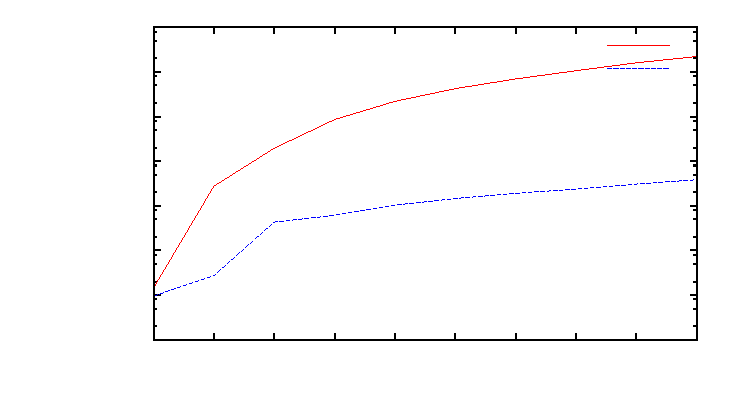
\includegraphics{texplots/gc_big_010}}%
    \gplfronttext
  \end{picture}%
\endgroup

\caption{Densidad $p = 0.1$}
\end{figure}

\begin{figure}[H]
\centering
% GNUPLOT: LaTeX picture with Postscript
\begingroup
  \makeatletter
  \providecommand\color[2][]{%
    \GenericError{(gnuplot) \space\space\space\@spaces}{%
      Package color not loaded in conjunction with
      terminal option `colourtext'%
    }{See the gnuplot documentation for explanation.%
    }{Either use 'blacktext' in gnuplot or load the package
      color.sty in LaTeX.}%
    \renewcommand\color[2][]{}%
  }%
  \providecommand\includegraphics[2][]{%
    \GenericError{(gnuplot) \space\space\space\@spaces}{%
      Package graphicx or graphics not loaded%
    }{See the gnuplot documentation for explanation.%
    }{The gnuplot epslatex terminal needs graphicx.sty or graphics.sty.}%
    \renewcommand\includegraphics[2][]{}%
  }%
  \providecommand\rotatebox[2]{#2}%
  \@ifundefined{ifGPcolor}{%
    \newif\ifGPcolor
    \GPcolorfalse
  }{}%
  \@ifundefined{ifGPblacktext}{%
    \newif\ifGPblacktext
    \GPblacktexttrue
  }{}%
  % define a \g@addto@macro without @ in the name:
  \let\gplgaddtomacro\g@addto@macro
  % define empty templates for all commands taking text:
  \gdef\gplbacktext{}%
  \gdef\gplfronttext{}%
  \makeatother
  \ifGPblacktext
    % no textcolor at all
    \def\colorrgb#1{}%
    \def\colorgray#1{}%
  \else
    % gray or color?
    \ifGPcolor
      \def\colorrgb#1{\color[rgb]{#1}}%
      \def\colorgray#1{\color[gray]{#1}}%
      \expandafter\def\csname LTw\endcsname{\color{white}}%
      \expandafter\def\csname LTb\endcsname{\color{black}}%
      \expandafter\def\csname LTa\endcsname{\color{black}}%
      \expandafter\def\csname LT0\endcsname{\color[rgb]{1,0,0}}%
      \expandafter\def\csname LT1\endcsname{\color[rgb]{0,1,0}}%
      \expandafter\def\csname LT2\endcsname{\color[rgb]{0,0,1}}%
      \expandafter\def\csname LT3\endcsname{\color[rgb]{1,0,1}}%
      \expandafter\def\csname LT4\endcsname{\color[rgb]{0,1,1}}%
      \expandafter\def\csname LT5\endcsname{\color[rgb]{1,1,0}}%
      \expandafter\def\csname LT6\endcsname{\color[rgb]{0,0,0}}%
      \expandafter\def\csname LT7\endcsname{\color[rgb]{1,0.3,0}}%
      \expandafter\def\csname LT8\endcsname{\color[rgb]{0.5,0.5,0.5}}%
    \else
      % gray
      \def\colorrgb#1{\color{black}}%
      \def\colorgray#1{\color[gray]{#1}}%
      \expandafter\def\csname LTw\endcsname{\color{white}}%
      \expandafter\def\csname LTb\endcsname{\color{black}}%
      \expandafter\def\csname LTa\endcsname{\color{black}}%
      \expandafter\def\csname LT0\endcsname{\color{black}}%
      \expandafter\def\csname LT1\endcsname{\color{black}}%
      \expandafter\def\csname LT2\endcsname{\color{black}}%
      \expandafter\def\csname LT3\endcsname{\color{black}}%
      \expandafter\def\csname LT4\endcsname{\color{black}}%
      \expandafter\def\csname LT5\endcsname{\color{black}}%
      \expandafter\def\csname LT6\endcsname{\color{black}}%
      \expandafter\def\csname LT7\endcsname{\color{black}}%
      \expandafter\def\csname LT8\endcsname{\color{black}}%
    \fi
  \fi
  \setlength{\unitlength}{0.0500bp}%
  \begin{picture}(7086.00,3968.00)%
    \gplgaddtomacro\gplbacktext{%
      \csname LTb\endcsname%
      \put(1210,704){\makebox(0,0)[r]{\strut{} 1e+06}}%
      \put(1210,1204){\makebox(0,0)[r]{\strut{} 1e+07}}%
      \put(1210,1704){\makebox(0,0)[r]{\strut{} 1e+08}}%
      \put(1210,2204){\makebox(0,0)[r]{\strut{} 1e+09}}%
      \put(1210,2703){\makebox(0,0)[r]{\strut{} 1e+10}}%
      \put(1210,3203){\makebox(0,0)[r]{\strut{} 1e+11}}%
      \put(1210,3703){\makebox(0,0)[r]{\strut{} 1e+12}}%
      \put(1342,484){\makebox(0,0){\strut{} 500}}%
      \put(1936,484){\makebox(0,0){\strut{} 1000}}%
      \put(2530,484){\makebox(0,0){\strut{} 1500}}%
      \put(3124,484){\makebox(0,0){\strut{} 2000}}%
      \put(3718,484){\makebox(0,0){\strut{} 2500}}%
      \put(4313,484){\makebox(0,0){\strut{} 3000}}%
      \put(4907,484){\makebox(0,0){\strut{} 3500}}%
      \put(5501,484){\makebox(0,0){\strut{} 4000}}%
      \put(6095,484){\makebox(0,0){\strut{} 4500}}%
      \put(6689,484){\makebox(0,0){\strut{} 5000}}%
      \put(176,2203){\rotatebox{-270}{\makebox(0,0){\strut{}TSC}}}%
      \put(4015,154){\makebox(0,0){\strut{}Cantidad de nodos ($n$)}}%
    }%
    \gplgaddtomacro\gplfronttext{%
      \csname LTb\endcsname%
      \put(5702,3530){\makebox(0,0)[r]{\strut{}Estándar}}%
      \csname LTb\endcsname%
      \put(5702,3310){\makebox(0,0)[r]{\strut{}Con conjunto de direcciones}}%
    }%
    \gplbacktext
    \put(0,0){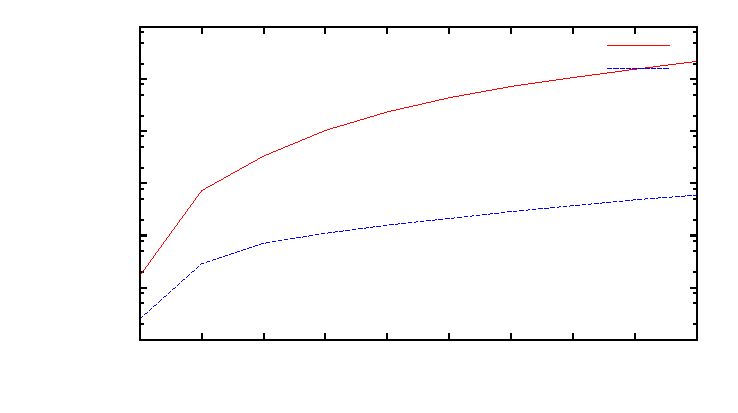
\includegraphics{texplots/gc_big_025}}%
    \gplfronttext
  \end{picture}%
\endgroup

\caption{Densidad $p = 0.25$}
\end{figure}

\begin{figure}[H]
\centering
% GNUPLOT: LaTeX picture with Postscript
\begingroup
  \makeatletter
  \providecommand\color[2][]{%
    \GenericError{(gnuplot) \space\space\space\@spaces}{%
      Package color not loaded in conjunction with
      terminal option `colourtext'%
    }{See the gnuplot documentation for explanation.%
    }{Either use 'blacktext' in gnuplot or load the package
      color.sty in LaTeX.}%
    \renewcommand\color[2][]{}%
  }%
  \providecommand\includegraphics[2][]{%
    \GenericError{(gnuplot) \space\space\space\@spaces}{%
      Package graphicx or graphics not loaded%
    }{See the gnuplot documentation for explanation.%
    }{The gnuplot epslatex terminal needs graphicx.sty or graphics.sty.}%
    \renewcommand\includegraphics[2][]{}%
  }%
  \providecommand\rotatebox[2]{#2}%
  \@ifundefined{ifGPcolor}{%
    \newif\ifGPcolor
    \GPcolorfalse
  }{}%
  \@ifundefined{ifGPblacktext}{%
    \newif\ifGPblacktext
    \GPblacktexttrue
  }{}%
  % define a \g@addto@macro without @ in the name:
  \let\gplgaddtomacro\g@addto@macro
  % define empty templates for all commands taking text:
  \gdef\gplbacktext{}%
  \gdef\gplfronttext{}%
  \makeatother
  \ifGPblacktext
    % no textcolor at all
    \def\colorrgb#1{}%
    \def\colorgray#1{}%
  \else
    % gray or color?
    \ifGPcolor
      \def\colorrgb#1{\color[rgb]{#1}}%
      \def\colorgray#1{\color[gray]{#1}}%
      \expandafter\def\csname LTw\endcsname{\color{white}}%
      \expandafter\def\csname LTb\endcsname{\color{black}}%
      \expandafter\def\csname LTa\endcsname{\color{black}}%
      \expandafter\def\csname LT0\endcsname{\color[rgb]{1,0,0}}%
      \expandafter\def\csname LT1\endcsname{\color[rgb]{0,1,0}}%
      \expandafter\def\csname LT2\endcsname{\color[rgb]{0,0,1}}%
      \expandafter\def\csname LT3\endcsname{\color[rgb]{1,0,1}}%
      \expandafter\def\csname LT4\endcsname{\color[rgb]{0,1,1}}%
      \expandafter\def\csname LT5\endcsname{\color[rgb]{1,1,0}}%
      \expandafter\def\csname LT6\endcsname{\color[rgb]{0,0,0}}%
      \expandafter\def\csname LT7\endcsname{\color[rgb]{1,0.3,0}}%
      \expandafter\def\csname LT8\endcsname{\color[rgb]{0.5,0.5,0.5}}%
    \else
      % gray
      \def\colorrgb#1{\color{black}}%
      \def\colorgray#1{\color[gray]{#1}}%
      \expandafter\def\csname LTw\endcsname{\color{white}}%
      \expandafter\def\csname LTb\endcsname{\color{black}}%
      \expandafter\def\csname LTa\endcsname{\color{black}}%
      \expandafter\def\csname LT0\endcsname{\color{black}}%
      \expandafter\def\csname LT1\endcsname{\color{black}}%
      \expandafter\def\csname LT2\endcsname{\color{black}}%
      \expandafter\def\csname LT3\endcsname{\color{black}}%
      \expandafter\def\csname LT4\endcsname{\color{black}}%
      \expandafter\def\csname LT5\endcsname{\color{black}}%
      \expandafter\def\csname LT6\endcsname{\color{black}}%
      \expandafter\def\csname LT7\endcsname{\color{black}}%
      \expandafter\def\csname LT8\endcsname{\color{black}}%
    \fi
  \fi
  \setlength{\unitlength}{0.0500bp}%
  \begin{picture}(7086.00,3968.00)%
    \gplgaddtomacro\gplbacktext{%
      \csname LTb\endcsname%
      \put(1210,704){\makebox(0,0)[r]{\strut{} 1e+07}}%
      \put(1210,1304){\makebox(0,0)[r]{\strut{} 1e+08}}%
      \put(1210,1904){\makebox(0,0)[r]{\strut{} 1e+09}}%
      \put(1210,2503){\makebox(0,0)[r]{\strut{} 1e+10}}%
      \put(1210,3103){\makebox(0,0)[r]{\strut{} 1e+11}}%
      \put(1210,3703){\makebox(0,0)[r]{\strut{} 1e+12}}%
      \put(1342,484){\makebox(0,0){\strut{} 500}}%
      \put(1936,484){\makebox(0,0){\strut{} 1000}}%
      \put(2530,484){\makebox(0,0){\strut{} 1500}}%
      \put(3124,484){\makebox(0,0){\strut{} 2000}}%
      \put(3718,484){\makebox(0,0){\strut{} 2500}}%
      \put(4313,484){\makebox(0,0){\strut{} 3000}}%
      \put(4907,484){\makebox(0,0){\strut{} 3500}}%
      \put(5501,484){\makebox(0,0){\strut{} 4000}}%
      \put(6095,484){\makebox(0,0){\strut{} 4500}}%
      \put(6689,484){\makebox(0,0){\strut{} 5000}}%
      \put(176,2203){\rotatebox{-270}{\makebox(0,0){\strut{}TSC}}}%
      \put(4015,154){\makebox(0,0){\strut{}Cantidad de nodos ($n$)}}%
    }%
    \gplgaddtomacro\gplfronttext{%
      \csname LTb\endcsname%
      \put(5702,3530){\makebox(0,0)[r]{\strut{}Estándar}}%
      \csname LTb\endcsname%
      \put(5702,3310){\makebox(0,0)[r]{\strut{}Con conjunto de direcciones}}%
    }%
    \gplbacktext
    \put(0,0){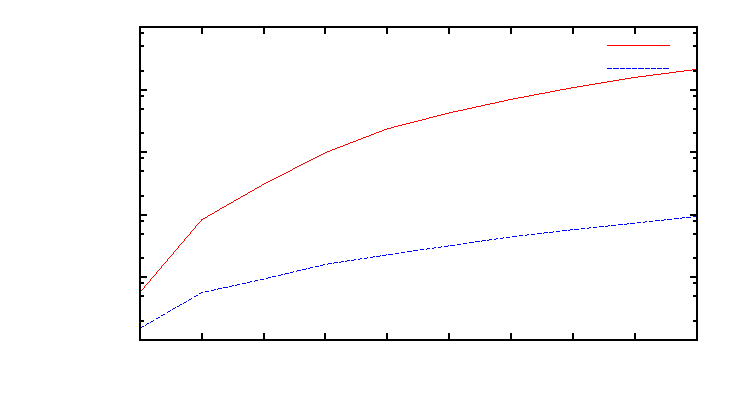
\includegraphics{texplots/gc_big_050}}%
    \gplfronttext
  \end{picture}%
\endgroup

\caption{Densidad $p = 0.5$}
\end{figure}

\begin{figure}[H]
\centering
% GNUPLOT: LaTeX picture with Postscript
\begingroup
  \makeatletter
  \providecommand\color[2][]{%
    \GenericError{(gnuplot) \space\space\space\@spaces}{%
      Package color not loaded in conjunction with
      terminal option `colourtext'%
    }{See the gnuplot documentation for explanation.%
    }{Either use 'blacktext' in gnuplot or load the package
      color.sty in LaTeX.}%
    \renewcommand\color[2][]{}%
  }%
  \providecommand\includegraphics[2][]{%
    \GenericError{(gnuplot) \space\space\space\@spaces}{%
      Package graphicx or graphics not loaded%
    }{See the gnuplot documentation for explanation.%
    }{The gnuplot epslatex terminal needs graphicx.sty or graphics.sty.}%
    \renewcommand\includegraphics[2][]{}%
  }%
  \providecommand\rotatebox[2]{#2}%
  \@ifundefined{ifGPcolor}{%
    \newif\ifGPcolor
    \GPcolorfalse
  }{}%
  \@ifundefined{ifGPblacktext}{%
    \newif\ifGPblacktext
    \GPblacktexttrue
  }{}%
  % define a \g@addto@macro without @ in the name:
  \let\gplgaddtomacro\g@addto@macro
  % define empty templates for all commands taking text:
  \gdef\gplbacktext{}%
  \gdef\gplfronttext{}%
  \makeatother
  \ifGPblacktext
    % no textcolor at all
    \def\colorrgb#1{}%
    \def\colorgray#1{}%
  \else
    % gray or color?
    \ifGPcolor
      \def\colorrgb#1{\color[rgb]{#1}}%
      \def\colorgray#1{\color[gray]{#1}}%
      \expandafter\def\csname LTw\endcsname{\color{white}}%
      \expandafter\def\csname LTb\endcsname{\color{black}}%
      \expandafter\def\csname LTa\endcsname{\color{black}}%
      \expandafter\def\csname LT0\endcsname{\color[rgb]{1,0,0}}%
      \expandafter\def\csname LT1\endcsname{\color[rgb]{0,1,0}}%
      \expandafter\def\csname LT2\endcsname{\color[rgb]{0,0,1}}%
      \expandafter\def\csname LT3\endcsname{\color[rgb]{1,0,1}}%
      \expandafter\def\csname LT4\endcsname{\color[rgb]{0,1,1}}%
      \expandafter\def\csname LT5\endcsname{\color[rgb]{1,1,0}}%
      \expandafter\def\csname LT6\endcsname{\color[rgb]{0,0,0}}%
      \expandafter\def\csname LT7\endcsname{\color[rgb]{1,0.3,0}}%
      \expandafter\def\csname LT8\endcsname{\color[rgb]{0.5,0.5,0.5}}%
    \else
      % gray
      \def\colorrgb#1{\color{black}}%
      \def\colorgray#1{\color[gray]{#1}}%
      \expandafter\def\csname LTw\endcsname{\color{white}}%
      \expandafter\def\csname LTb\endcsname{\color{black}}%
      \expandafter\def\csname LTa\endcsname{\color{black}}%
      \expandafter\def\csname LT0\endcsname{\color{black}}%
      \expandafter\def\csname LT1\endcsname{\color{black}}%
      \expandafter\def\csname LT2\endcsname{\color{black}}%
      \expandafter\def\csname LT3\endcsname{\color{black}}%
      \expandafter\def\csname LT4\endcsname{\color{black}}%
      \expandafter\def\csname LT5\endcsname{\color{black}}%
      \expandafter\def\csname LT6\endcsname{\color{black}}%
      \expandafter\def\csname LT7\endcsname{\color{black}}%
      \expandafter\def\csname LT8\endcsname{\color{black}}%
    \fi
  \fi
  \setlength{\unitlength}{0.0500bp}%
  \begin{picture}(7086.00,3968.00)%
    \gplgaddtomacro\gplbacktext{%
      \csname LTb\endcsname%
      \put(1210,704){\makebox(0,0)[r]{\strut{} 1e+07}}%
      \put(1210,1304){\makebox(0,0)[r]{\strut{} 1e+08}}%
      \put(1210,1904){\makebox(0,0)[r]{\strut{} 1e+09}}%
      \put(1210,2503){\makebox(0,0)[r]{\strut{} 1e+10}}%
      \put(1210,3103){\makebox(0,0)[r]{\strut{} 1e+11}}%
      \put(1210,3703){\makebox(0,0)[r]{\strut{} 1e+12}}%
      \put(1342,484){\makebox(0,0){\strut{} 500}}%
      \put(1936,484){\makebox(0,0){\strut{} 1000}}%
      \put(2530,484){\makebox(0,0){\strut{} 1500}}%
      \put(3124,484){\makebox(0,0){\strut{} 2000}}%
      \put(3718,484){\makebox(0,0){\strut{} 2500}}%
      \put(4313,484){\makebox(0,0){\strut{} 3000}}%
      \put(4907,484){\makebox(0,0){\strut{} 3500}}%
      \put(5501,484){\makebox(0,0){\strut{} 4000}}%
      \put(6095,484){\makebox(0,0){\strut{} 4500}}%
      \put(6689,484){\makebox(0,0){\strut{} 5000}}%
      \put(176,2203){\rotatebox{-270}{\makebox(0,0){\strut{}TSC}}}%
      \put(4015,154){\makebox(0,0){\strut{}Cantidad de nodos ($n$)}}%
    }%
    \gplgaddtomacro\gplfronttext{%
      \csname LTb\endcsname%
      \put(5702,3530){\makebox(0,0)[r]{\strut{}Estándar}}%
      \csname LTb\endcsname%
      \put(5702,3310){\makebox(0,0)[r]{\strut{}Con conjunto de direcciones}}%
    }%
    \gplbacktext
    \put(0,0){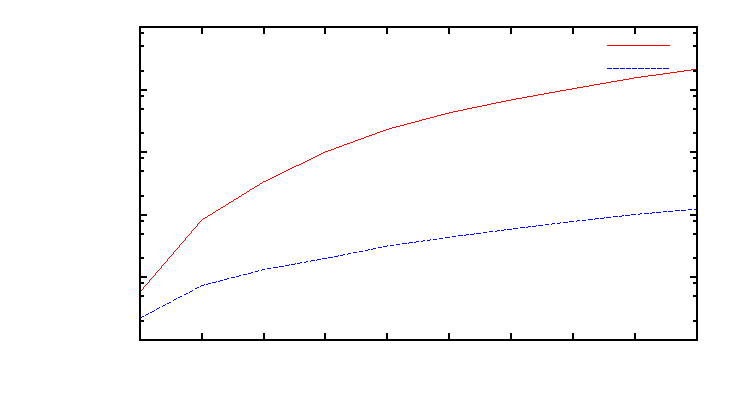
\includegraphics{texplots/gc_big_075}}%
    \gplfronttext
  \end{picture}%
\endgroup

\caption{Densidad $p = 0.75$}
\end{figure}

\begin{figure}[H]
\centering
% GNUPLOT: LaTeX picture with Postscript
\begingroup
  \makeatletter
  \providecommand\color[2][]{%
    \GenericError{(gnuplot) \space\space\space\@spaces}{%
      Package color not loaded in conjunction with
      terminal option `colourtext'%
    }{See the gnuplot documentation for explanation.%
    }{Either use 'blacktext' in gnuplot or load the package
      color.sty in LaTeX.}%
    \renewcommand\color[2][]{}%
  }%
  \providecommand\includegraphics[2][]{%
    \GenericError{(gnuplot) \space\space\space\@spaces}{%
      Package graphicx or graphics not loaded%
    }{See the gnuplot documentation for explanation.%
    }{The gnuplot epslatex terminal needs graphicx.sty or graphics.sty.}%
    \renewcommand\includegraphics[2][]{}%
  }%
  \providecommand\rotatebox[2]{#2}%
  \@ifundefined{ifGPcolor}{%
    \newif\ifGPcolor
    \GPcolorfalse
  }{}%
  \@ifundefined{ifGPblacktext}{%
    \newif\ifGPblacktext
    \GPblacktexttrue
  }{}%
  % define a \g@addto@macro without @ in the name:
  \let\gplgaddtomacro\g@addto@macro
  % define empty templates for all commands taking text:
  \gdef\gplbacktext{}%
  \gdef\gplfronttext{}%
  \makeatother
  \ifGPblacktext
    % no textcolor at all
    \def\colorrgb#1{}%
    \def\colorgray#1{}%
  \else
    % gray or color?
    \ifGPcolor
      \def\colorrgb#1{\color[rgb]{#1}}%
      \def\colorgray#1{\color[gray]{#1}}%
      \expandafter\def\csname LTw\endcsname{\color{white}}%
      \expandafter\def\csname LTb\endcsname{\color{black}}%
      \expandafter\def\csname LTa\endcsname{\color{black}}%
      \expandafter\def\csname LT0\endcsname{\color[rgb]{1,0,0}}%
      \expandafter\def\csname LT1\endcsname{\color[rgb]{0,1,0}}%
      \expandafter\def\csname LT2\endcsname{\color[rgb]{0,0,1}}%
      \expandafter\def\csname LT3\endcsname{\color[rgb]{1,0,1}}%
      \expandafter\def\csname LT4\endcsname{\color[rgb]{0,1,1}}%
      \expandafter\def\csname LT5\endcsname{\color[rgb]{1,1,0}}%
      \expandafter\def\csname LT6\endcsname{\color[rgb]{0,0,0}}%
      \expandafter\def\csname LT7\endcsname{\color[rgb]{1,0.3,0}}%
      \expandafter\def\csname LT8\endcsname{\color[rgb]{0.5,0.5,0.5}}%
    \else
      % gray
      \def\colorrgb#1{\color{black}}%
      \def\colorgray#1{\color[gray]{#1}}%
      \expandafter\def\csname LTw\endcsname{\color{white}}%
      \expandafter\def\csname LTb\endcsname{\color{black}}%
      \expandafter\def\csname LTa\endcsname{\color{black}}%
      \expandafter\def\csname LT0\endcsname{\color{black}}%
      \expandafter\def\csname LT1\endcsname{\color{black}}%
      \expandafter\def\csname LT2\endcsname{\color{black}}%
      \expandafter\def\csname LT3\endcsname{\color{black}}%
      \expandafter\def\csname LT4\endcsname{\color{black}}%
      \expandafter\def\csname LT5\endcsname{\color{black}}%
      \expandafter\def\csname LT6\endcsname{\color{black}}%
      \expandafter\def\csname LT7\endcsname{\color{black}}%
      \expandafter\def\csname LT8\endcsname{\color{black}}%
    \fi
  \fi
  \setlength{\unitlength}{0.0500bp}%
  \begin{picture}(7086.00,3968.00)%
    \gplgaddtomacro\gplbacktext{%
      \csname LTb\endcsname%
      \put(1210,704){\makebox(0,0)[r]{\strut{} 1e+07}}%
      \put(1210,1304){\makebox(0,0)[r]{\strut{} 1e+08}}%
      \put(1210,1904){\makebox(0,0)[r]{\strut{} 1e+09}}%
      \put(1210,2503){\makebox(0,0)[r]{\strut{} 1e+10}}%
      \put(1210,3103){\makebox(0,0)[r]{\strut{} 1e+11}}%
      \put(1210,3703){\makebox(0,0)[r]{\strut{} 1e+12}}%
      \put(1342,484){\makebox(0,0){\strut{} 500}}%
      \put(1936,484){\makebox(0,0){\strut{} 1000}}%
      \put(2530,484){\makebox(0,0){\strut{} 1500}}%
      \put(3124,484){\makebox(0,0){\strut{} 2000}}%
      \put(3718,484){\makebox(0,0){\strut{} 2500}}%
      \put(4313,484){\makebox(0,0){\strut{} 3000}}%
      \put(4907,484){\makebox(0,0){\strut{} 3500}}%
      \put(5501,484){\makebox(0,0){\strut{} 4000}}%
      \put(6095,484){\makebox(0,0){\strut{} 4500}}%
      \put(6689,484){\makebox(0,0){\strut{} 5000}}%
      \put(176,2203){\rotatebox{-270}{\makebox(0,0){\strut{}TSC}}}%
      \put(4015,154){\makebox(0,0){\strut{}Cantidad de nodos ($n$)}}%
    }%
    \gplgaddtomacro\gplfronttext{%
      \csname LTb\endcsname%
      \put(5702,3530){\makebox(0,0)[r]{\strut{}Estándar}}%
      \csname LTb\endcsname%
      \put(5702,3310){\makebox(0,0)[r]{\strut{}Con conjunto de direcciones}}%
    }%
    \gplbacktext
    \put(0,0){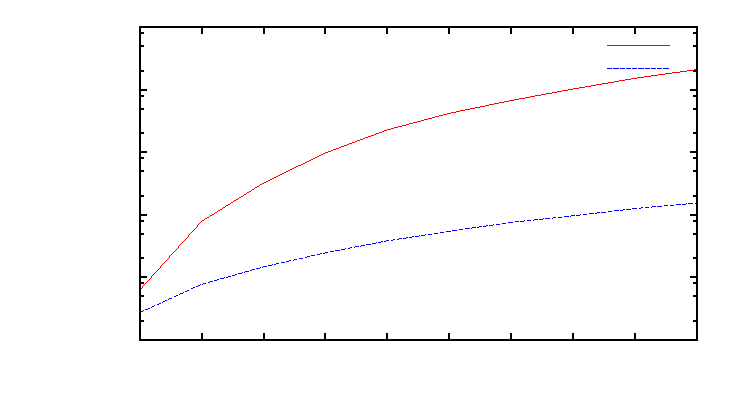
\includegraphics{texplots/gc_big_100}}%
    \gplfronttext
  \end{picture}%
\endgroup

\caption{Densidad $p = 1$}
\end{figure}

Notar que todas las escalas son logarítmicas. La diferencia de tiempos entre ambas versiones es muy grande, siendo el Mark-Sweep con conjunto de direcciones, en promedio, 100 veces más rápida que el estándar.

Se puede observar que la versión estándar no es suceptible ante variaciones en la densidad del grafo de objetos. Esto es coherente con el hecho de que la función es $\Omega(n^2 \cdot size)$ (lo cual se deduce de un análisis de la complejidad análogo al realizado antes) y en consecuencia $\Theta(n^2 \cdot size)$, complejidad que es independiente del valor de $m$. Contrariamente, la versión de Mark-Sweep con conjunto de direcciones se ve afectada por la densidad (observar la diferencia de crecimento entre las curvas de las mediciones para $p = 0.1$ y $p = 0.25$). Esto se debe a que tal función es $\Theta(m + n \cdot size)$, dependiente de $m$.

Medimos además, para la versión con conjunto de direcciones, la memoria que ocupaba el trie representando dicho conjunto. Esta cantidad de memoria depende de varios factores. En primer lugar, depende de cuáles son las direcciones que almacenemos, pues un prefijo común de dos o más direcciones sólo es almacenado una vez en el trie. Claramente, también depende de la cantidad total de direcciones (igual a la cantidad de objetos). En cierta forma, depende del tamaño $size$ de un objeto cualquiera, ya que si los objetos son pequeños y contíguos en memoria entonces sus direcciones en memoria serán similares. Contrariamente, no depende de la densidad del grafo de objetos, pues el conjunto sólo almacena la dirección de cada objeto (de cada nodo del grafo), pero no su vínculo con otros objetos (aristas del grafo). La Figura \ref{fig:memoria} muestra el requerimiento de memoria promedio para cada tamaño del grafo de objetos.

\begin{figure}[H]
\centering
% GNUPLOT: LaTeX picture with Postscript
\begingroup
  \makeatletter
  \providecommand\color[2][]{%
    \GenericError{(gnuplot) \space\space\space\@spaces}{%
      Package color not loaded in conjunction with
      terminal option `colourtext'%
    }{See the gnuplot documentation for explanation.%
    }{Either use 'blacktext' in gnuplot or load the package
      color.sty in LaTeX.}%
    \renewcommand\color[2][]{}%
  }%
  \providecommand\includegraphics[2][]{%
    \GenericError{(gnuplot) \space\space\space\@spaces}{%
      Package graphicx or graphics not loaded%
    }{See the gnuplot documentation for explanation.%
    }{The gnuplot epslatex terminal needs graphicx.sty or graphics.sty.}%
    \renewcommand\includegraphics[2][]{}%
  }%
  \providecommand\rotatebox[2]{#2}%
  \@ifundefined{ifGPcolor}{%
    \newif\ifGPcolor
    \GPcolorfalse
  }{}%
  \@ifundefined{ifGPblacktext}{%
    \newif\ifGPblacktext
    \GPblacktexttrue
  }{}%
  % define a \g@addto@macro without @ in the name:
  \let\gplgaddtomacro\g@addto@macro
  % define empty templates for all commands taking text:
  \gdef\gplbacktext{}%
  \gdef\gplfronttext{}%
  \makeatother
  \ifGPblacktext
    % no textcolor at all
    \def\colorrgb#1{}%
    \def\colorgray#1{}%
  \else
    % gray or color?
    \ifGPcolor
      \def\colorrgb#1{\color[rgb]{#1}}%
      \def\colorgray#1{\color[gray]{#1}}%
      \expandafter\def\csname LTw\endcsname{\color{white}}%
      \expandafter\def\csname LTb\endcsname{\color{black}}%
      \expandafter\def\csname LTa\endcsname{\color{black}}%
      \expandafter\def\csname LT0\endcsname{\color[rgb]{1,0,0}}%
      \expandafter\def\csname LT1\endcsname{\color[rgb]{0,1,0}}%
      \expandafter\def\csname LT2\endcsname{\color[rgb]{0,0,1}}%
      \expandafter\def\csname LT3\endcsname{\color[rgb]{1,0,1}}%
      \expandafter\def\csname LT4\endcsname{\color[rgb]{0,1,1}}%
      \expandafter\def\csname LT5\endcsname{\color[rgb]{1,1,0}}%
      \expandafter\def\csname LT6\endcsname{\color[rgb]{0,0,0}}%
      \expandafter\def\csname LT7\endcsname{\color[rgb]{1,0.3,0}}%
      \expandafter\def\csname LT8\endcsname{\color[rgb]{0.5,0.5,0.5}}%
    \else
      % gray
      \def\colorrgb#1{\color{black}}%
      \def\colorgray#1{\color[gray]{#1}}%
      \expandafter\def\csname LTw\endcsname{\color{white}}%
      \expandafter\def\csname LTb\endcsname{\color{black}}%
      \expandafter\def\csname LTa\endcsname{\color{black}}%
      \expandafter\def\csname LT0\endcsname{\color{black}}%
      \expandafter\def\csname LT1\endcsname{\color{black}}%
      \expandafter\def\csname LT2\endcsname{\color{black}}%
      \expandafter\def\csname LT3\endcsname{\color{black}}%
      \expandafter\def\csname LT4\endcsname{\color{black}}%
      \expandafter\def\csname LT5\endcsname{\color{black}}%
      \expandafter\def\csname LT6\endcsname{\color{black}}%
      \expandafter\def\csname LT7\endcsname{\color{black}}%
      \expandafter\def\csname LT8\endcsname{\color{black}}%
    \fi
  \fi
  \setlength{\unitlength}{0.0500bp}%
  \begin{picture}(7086.00,3968.00)%
    \gplgaddtomacro\gplbacktext{%
      \csname LTb\endcsname%
      \put(1342,704){\makebox(0,0)[r]{\strut{} 0}}%
      \put(1342,1079){\makebox(0,0)[r]{\strut{} 50000}}%
      \put(1342,1454){\makebox(0,0)[r]{\strut{} 100000}}%
      \put(1342,1829){\makebox(0,0)[r]{\strut{} 150000}}%
      \put(1342,2204){\makebox(0,0)[r]{\strut{} 200000}}%
      \put(1342,2578){\makebox(0,0)[r]{\strut{} 250000}}%
      \put(1342,2953){\makebox(0,0)[r]{\strut{} 300000}}%
      \put(1342,3328){\makebox(0,0)[r]{\strut{} 350000}}%
      \put(1342,3703){\makebox(0,0)[r]{\strut{} 400000}}%
      \put(1474,484){\makebox(0,0){\strut{} 500}}%
      \put(2053,484){\makebox(0,0){\strut{} 1000}}%
      \put(2633,484){\makebox(0,0){\strut{} 1500}}%
      \put(3212,484){\makebox(0,0){\strut{} 2000}}%
      \put(3792,484){\makebox(0,0){\strut{} 2500}}%
      \put(4371,484){\makebox(0,0){\strut{} 3000}}%
      \put(4951,484){\makebox(0,0){\strut{} 3500}}%
      \put(5530,484){\makebox(0,0){\strut{} 4000}}%
      \put(6110,484){\makebox(0,0){\strut{} 4500}}%
      \put(6689,484){\makebox(0,0){\strut{} 5000}}%
      \put(176,2203){\rotatebox{-270}{\makebox(0,0){\strut{}Tamaño en memoria del conjunto (B)}}}%
      \put(4081,154){\makebox(0,0){\strut{}Cantidad de nodos ($n$)}}%
    }%
    \gplgaddtomacro\gplfronttext{%
      \csname LTb\endcsname%
      \put(5702,3530){\makebox(0,0)[r]{\strut{}Con conjunto de direcciones}}%
    }%
    \gplbacktext
    \put(0,0){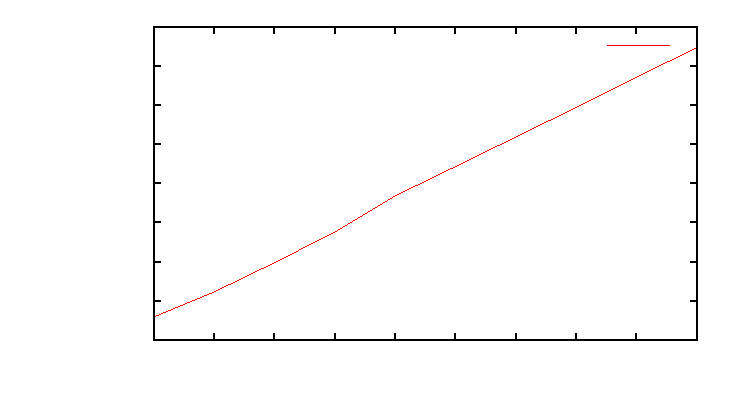
\includegraphics{texplots/gc_big_fast_memory}}%
    \gplfronttext
  \end{picture}%
\endgroup

\caption{Memoria requerida por la versión con conjunto}
\label{fig:memoria}
\end{figure}

Se puede ver que la memoria necesaria crece en forma aproximadamente lineal en la cantidad de objetos. Para 1000 objetos (u 80000B $\approx$ 80kB) , la memoria necesaria es aproximadamente 50kB. Para 2500 objetos (o 500000B $\approx$ 500kB), el requerimiento es de casi 200KB. Para 5000 objetos (o 2000000B $\approx$ 2000kB), el tamaño en memoria termina siendo un poco más de 350kB. Notemos que a medida que la cantidad de objetos crece, el espacio requerido por el conjunto se vuelve despreciable respecto del espacio requerido por los objetos.

De todo este análisis podemos concluir que hay un notable trade-off entre costo espacial y temporal de una versión a la otra. Mientras que la versión estándar no usa memoria adicional aparte de la empleada por la pila de memoria a lo largo de las llamadas recursivas, es 100 veces más lenta que la versión con conjunto de direcciones, pese a que esta última requiere una notable cantidad de memoria adicional. Esta segunda versión, más rápida pero más costosa en términos espaciales, parece más adecuada en, al menos, dos situaciones:

\begin{itemize}
\item Cuando la velocidad de recolección es prioridad por sobre la memoria utilizada.

\item Cuando la cantidad de objetos en memoria es muy grande. En este caso, el tamaño del conjunto se vuelve despreciable con lo cual, en términos relativos, la memoria adicional requerida es poca.
\end{itemize}

En otros casos, la utilización de memoria adicional puede resultar inadmisible, haciendo preferible a la versión estándar.